\documentclass[10pt,a4paper]{article}
\usepackage[utf8]{inputenc}
\usepackage{amsmath}
\usepackage{amsfonts}
\usepackage{amssymb}
\usepackage{graphicx}
\usepackage{color}
\usepackage{float}
\usepackage{eurosym}
\usepackage{booktabs,tabularx}

\usepackage{fancyhdr}
 
\pagestyle{fancy}
\fancyhf{}
\rhead{Amsterdam university of applied sciences}
\lhead{Swarming: Framework}
\rfoot{Page \thepage}


\definecolor{codegreen}{rgb}{0,0.6,0}
\definecolor{codegray}{rgb}{0.5,0.5,0.5}
\definecolor{codepurple}{rgb}{0.58,0,0.82}
\definecolor{backcolour}{rgb}{0.95,0.95,0.92}
\usepackage{listings}
\lstdefinestyle{cstyle}{
    backgroundcolor=\color{backcolour},   
    commentstyle=\color{codegreen},
    keywordstyle=\color{magenta},
    numberstyle=\tiny\color{codegray},
    stringstyle=\color{codepurple},
    basicstyle=\footnotesize,
    breakatwhitespace=false,         
    breaklines=true,                 
    captionpos=b,                    
    keepspaces=true,                 
    numbers=left,                    
    numbersep=5pt,                  
    showspaces=false,                
    showstringspaces=false,
    showtabs=false,                  
    tabsize=2
}
\graphicspath{ {./images/} }

\begin{document}
\begin{titlepage}
    \centering
    \vfill
    {\Large
    Swarming\\
   
    {\small Research framework}\\
        
        \vskip2cm
        {\small M. van Wilgenburg, W. Mukhtar, E. van Splunter, M. Siekerman, T. Zaal and M. Visser}\\
    }    
    \vfill
%    \includegraphics[width=1\textwidth]{WireS4}
    
    \vfill
    \vfill
\end{titlepage}

\newpage

\listoffigures
\newpage

\listoftables
\newpage
\tableofcontents
\newpage


\section{Problem analysis}
Researcher have always been inspired by nature. When they looked at "social" insects like ants they discovered "swarming"\cite{swarmwiki} . The behaviour of one ant on its own seems illogical, but together they solve problems of great importance for the entire colony. These ants make us of the so called "trail laying" and "trail following" principle. Every ants lays a trail of pheromones, when a few ants walk back and forth to a food source. The one walking the shortest route will lay a more concentrated trail. The other ants will get attracted by the strongest trail, this way a positive feedback loop is created, which will make every ant walk the shortest route if given enough time. This is one example where relatively simple units, can achieve complex goals like path finding because they work together in a swarm. This principle is called "swarm intelligence"\cite{swarmintelligence}.

Swarming can have alot of up sides compared to the "classical" approach. A few are: quicker solution time, lower unit complexity and a greater fault tolerance\cite{swarmintelligence}. When for example one of the units breaks down, then will the other units still be able to complete the task. When this happens to one, more complex unit, this wont be the case. For these reasons its interesting to researching the applications of swarming.



\section{Context analysis}
The Delft university of technology started a program to research the applications of swarming. In this program multiple universities work together to make this research possible. The idea of this program is that each project group contributes a small bit to reach the end result, which will be a working swarm of robots. The technology developed should be modular, so it can be easily used on other platforms.\\The programs focus lies on researching the applications of swarming on Mars. Its preferable that the technologies developed also work on Mars, but in some cases other technologies can be used to cut the cost. For example, for a simple proximity sensor on earth, an ultrasonic sensor would do just fine. But in the Mars atmosphere the ultrasonic waves get heavily dampened to the point where the sensor just wont work\cite{soundonmars}. The cheapest sensor that would work on Mars would be a lidar\cite{lidarmars}. While the average ultrasonic sensor costs around 2$\euro$ the cheapest lidar costs atleast 100$\euro$. In this project the aim is to build one unit for around 200$\euro$, just one lidar sensor would be half of the robots budget. To proof the concept of swarming the robots don't need to be "Mars proof", so costs will be cut where possible.\\

\section{Problem definition}
Swarming intelligent systems are typically made up of simple agents(robots) interacting locally with one another and their environment. The group of individuals acting in such manner is referred to as a swarm\cite{swarmintelligence}. For a group of robots to qualify as a swarm-robotics the following criteria have to be met:

\begin{itemize}
	\item Autonomy - It is required that the individuals that make up 	the swarm-robotic system are autonomous robots. They are able to 		physically 		interact with the environment and affect it.
	\item Large number - A large number of units is required
	as well, so the cooperative behavior (and
	swarm intelligence) may occur. The minimum number
	is hard to define and justify. The swarm-robotic
	system can be made of few homogeneous groups of
	robots consisted of large number of units. Highly heterogeneous
	robot groups tend to fall outside swarm
	robotics.
	\item Limited capabilities - The robots in a swarm
	should be relatively incapable or inefficien on their
	own with respect to the task at hand.
	\item Scalability and robustness - A swarm-robotic
	system needs to be scalable and robust. Adding the
	new units will improve the performance of the overall
	system and on the other hand, loosing some units will
	not cause the catastrophic failure.
	\item Distributed coordination - The robots in a swarm
	should only have local and limited sensing and communication
	abilities. The coordination between the
	robots is distributed. The use of a global channel for
	the coordination would influence the autonomy of the
	units.
\end{itemize}

These criteria are a good indication of what makes a system swarm-robotic. But should not be used to determine whether a system is swarm-robotic or not. This is because some criteria are still somewhat vague\cite{swarmintelligence}.Looking at these criteria we chose to define the problem into two sub-problems. This division is chosen because problem one will cover distributed coordination and scalability with what we call a "swarming module", which will provide communication and relative localization to the other units in the swarm. And problem two covers Autonomy, Large number and limited capabilities.  Problem two will cover the platform that will provide movement and some basic autonomous functions. The projects focus will be the swarming module. The swarming module has to be completely modular so it can easily be used on other robotic platforms in future projects. Because of this the commissioning party stresses that this has to be a finished product. Resources(time) should be focused on the swarming module. For the sake of demonstration, problem two (the robot platform) will also need to be developed. This platform will have to provide some basic autonomous functions like movement and obstacle avoidance. One important requirement is that it should be easily replicated, so a swarm of these platforms can be created.\\

\subsection{Goal}
As previously discussed the problem is now divided in two sub-problems with the focus on the swarming module. In this paragraph will be discussed what will be expected from the swarming module and the robot platform.

\subsubsection{Swarmingmodule}
Distributed coordination is one of the swarming criteria. To achieve this, some form of (relative) localization is needed. This should keep units from moving to close or to far from each other. And could also be used to accomplish certain goals like;  mapping, assembly of structures or inspections \cite{networkedRS}. Communication is needed to share information about the environment and every units position. Requirements here are that the communication should not be depended on one host and should be scalable. This is so communication is not cut off when one of the units breaks down. The scale-ability is important so that units can be added or removed from the swarm \cite{multidomaincom}. Because this project is part of a running program the modules made should be modular so they can be used on future projects. Summed up, the swarming module has the following characteristics.

\begin{itemize}
\item (Relative) Localization
\item Communication
\item Scalable
\item Modular
\end{itemize}

\subsubsection{Robot platform}
To properly demonstrate and test the swarming module, a robotic platform will be needed. This platform will need to meet the swarming criteria of autonomy, large numbers and limited capabilities. The autonomy of the robot should stay simple and robust, the key features are movement, obstacle avoidance and power supply. The robot has to be easily duplicated so multiple units can be produced for the swarm. Also it should be able to house the swarming module.

\newpage
\section{Research-question}

The main question of this research is as following: \textit{"How can communication and relative localization be achieved in a swarm or robots?".} To give an answer to this question there are multiple sub-questions to research first. 
 


\subsection{Sub-questions} 
The following questions need to be answered to come to a good conclusion to our research:

\begin{itemize}

    \item "What is swarming?"
    \begin{itemize}
        \item "What is the definition of swarming?"
        \item "How many robots are needed to create a swarm?"
        \item "How do the units communicate within the swarm?"
        \item "How do robots in the swarm know their location?"
    \end{itemize}    
    \item "Swarming communication"
    \begin{itemize}
        \item "What software protocol should be used?"
        \item "What hardware protocol should be used?"
        \item "What is de minimal required communication speed?"
        \item "What hardware is needed to implement the communication?"
    \end{itemize}
        \item "Communication between modules"
    \begin{itemize}
        \item "What software protocol should be used?"
        \item "What hardware protocol should be used?"
        \item "What is de minimal required communication speed?"
        \item "What hardware is needed to implement the communication?"
    \end{itemize}
    \item "What methods are there to propel the robot?"
    \begin{itemize}
        \item "What actuators can be used to drive the robot?"
        \item "How would the energy of the actuator be used to make the robot drive?"
        \item "What kind of effectors should be used?"
    \end{itemize}
    \item "What energy supply should be used to distribute the energy in the robot?"
    \begin{itemize}
        \item "How can the energy supply be managed?"
        \item "Is it possible to implement a recharge point?"
        \item "How can the energy supply be handled safely?"
    \end{itemize}
    \item "How will autonomous obstacle avoidance be achieved?"
    \begin{itemize}
   		 \item "What types of sensor technigues are there?"
    \end{itemize}
\end{itemize}
\newpage

\section{Specifications}
In this chapter the functional requirements for building a robot which can perform a task in cooperation with other robots will be defined. The specifications are divided into several features. The specifications to be achieved for swarming will be classified according to the MoSCoW-method. The corresponding specifications are further illustrated in this chapter. In the block diagram shown in Figure  \ref{fig:blockschematic}, the various modules are connected to each other.



\begin{figure}[h]
    \centering
    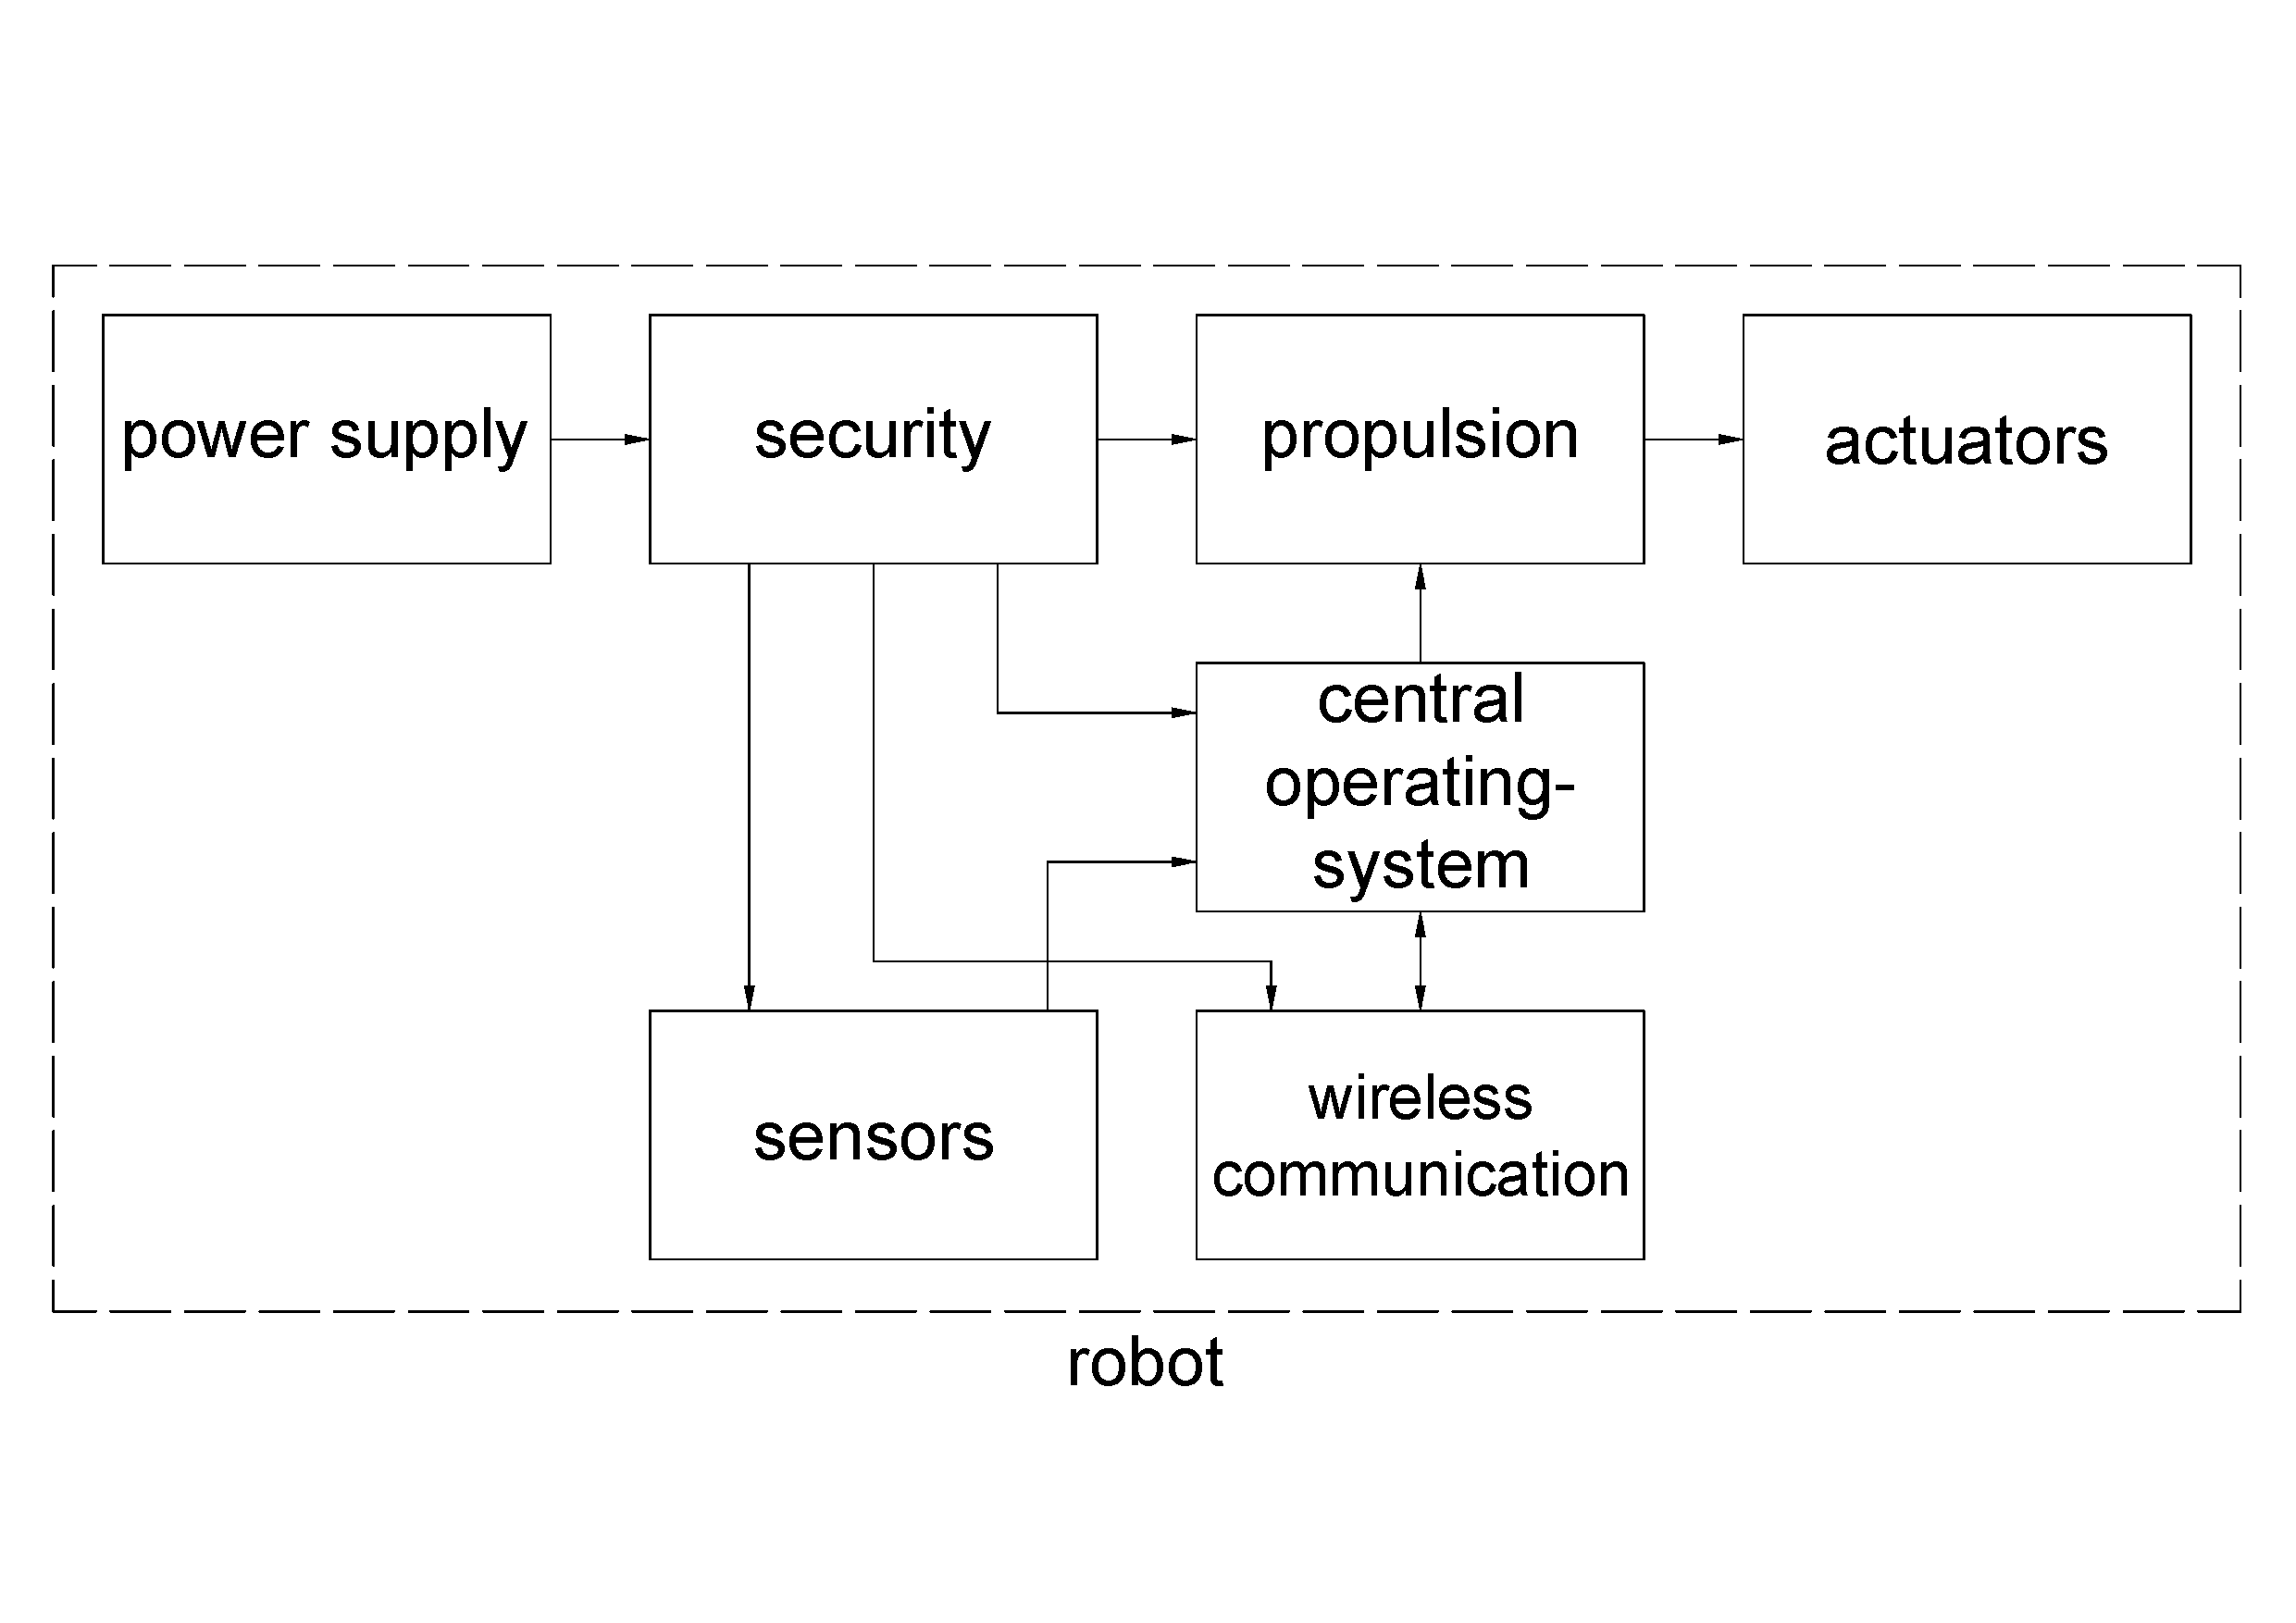
\includegraphics[width=1\textwidth]{blockschematic}
    \caption{simplified block diagram of the connection of the different subsystems within the robot }
    \label{fig:blockschematic}
\end{figure}



\subsection{Must haves}


M1 - Modular system architecture - Modules developed during this project must be modular so they can be used in future projects.\\\\
M2 - Units must be able to communicate with each other - The units in the swarm must be able to exchange information to properly funtion as a swarm. This is discussed in the problem defention\cite{multidomaincom}.  \\\\
M3 - Relative localization to other units - Localization is needed for robots to properly function in a swarm. This is discussed in the problem defention\cite{multidomaincom}\\\\
M4 - The communication needs to be wireless - The robots cant be restrained by wires, they need to be able to move freely trough their environment.\\\\
M5 - Scalable swarm population - This is one of the criteria of swarming discussed in the problem definition\\\\


\subsection{Should haves}

S1 - Is able to carry a payload - One criteria of swarming is that robots should be able to adjust their environment, a payload could be some kind of tool to make this possible\\\\
S2 - The robot platform must be modular - It would be preferable if the robots developed during this project are modular so they can be used in further development.\\\\
S3 - The robot must be able to propel themselves omnidirectional - For exploration based mission the robots should be able to move in different directions so the full area can be explored.\\

\subsection{Could haves}

C1 - Can move according to the principle of the ZebRo - Research shows that the ZebRo walking principle is a proven concept to get across rough terrain.\\\\
C2 - Ability to self- charging/ recharging of energy - Makes the robot capable of operating for a not determined time.\\\\
C3 - Shows signs of intelligence - Could learn how to behave on specific (environment) situations\\\\
C4 - Is aware when the robot is upside down - When the robot gets in a situation where it is unable to move, the orientation could be usefull to free itself. \\\\



\subsection{Won't haves}
\begin{itemize}
\item A master in the swarm network
\end{itemize}

\newpage

\section{Sub-specifications}

\begin{table}[H]
\centering
\caption{Sensors}
\label{Sensors}
\begin{tabular}{|l|l|}
\hline
Module    & Sensors \\ \hline
Input  & Communication with the system          \\ \hline
Output & Communication with the system             \\ \hline
Functions   & \begin{tabular}[c]{@{}l@{}}measuring the distance between itself and the environment\\ To communicate the measured value to the controller\end{tabular}            \\ \hline
\end{tabular}
\end{table}

The sensors on the robot must create awareness of its surroundings so that he can anticipate. See Table \ref{Sensors}\\

\begin{table}[H]
\centering
\caption{Power supply}
\label{supply}
\begin{tabular}{|l|l|}
\hline
Module    & Power supply \\ \hline
Input  & Power supply            \\ \hline
Output & Communication with the system             \\ \hline
Functions   & \begin{tabular}[c]{@{}l@{}}measuring the voltage/ current of the Power supply\\ To send the measured value to the controller\end{tabular}            \\ \hline
\end{tabular}
\end{table}


It is important to measure the battery level to ensure that the robots will not be able malfunction. \\The measured value is send to the controller. See Table \ref{supply}\\

\begin{table}[H]
\centering
\caption{Wireless communication mudule}
\label{communication}
\begin{tabular}{|l|l|}
\hline
Module    & Wireless communication mudule \\ \hline
Input  & \begin{tabular}[c]{@{}l@{}}Communication with the system\\ Communication with the other robots in the swarm          
\end{tabular}   \\ \hline
Output & \begin{tabular}[c]{@{}l@{}}Communication with the system\\ Communication with the other robots in the swarm         
\end{tabular}   \\ \hline
Functions   & \begin{tabular}[c]{@{}l@{}}establishes the communication between the modules swarm \\ Obtains information regarding the distance between the different robots\end{tabular}            \\ \hline
\end{tabular}
\end{table}


To communicate between different units a communication network should be set up with a common protocol . In addition, the protocol must be able to provide additional information such as localization. See Table \ref{communication} \\

\begin{table}[H]
\centering
\caption{effectors}
\label{Effectors}
\begin{tabular}{|l|l|}
\hline
Module    & Effectors \\ \hline
Input  & motor drivers  \\ \hline
Output & mechanical power   \\ \hline
Functions  & Drives the robot , and is able to turn on command            \\ \hline
\end{tabular}
\end{table}

The operator must , in addition to the functioning in the testenvironment , also function well on Mars . See Table \ref{Effectors} \\

\begin{table}[H]
\centering
\caption{Central control unit}
\label{control}
\begin{tabular}{|l|l|}
\hline
Module    & Central control unit \\ \hline
Input  & All information from the system  \\ \hline
Output & All control of the modules in the robot \\ \hline
Functions  & All the communication comes together and controls the inputs and outputs            \\ \hline
\end{tabular}
\end{table}

The central control unit handles all communication between the various modules that are present on the robot. See Table \ref{control}



\newpage
\subsection{Excising swarming Modules}

In this chapter existing swarming modules will be researched and reviewed.

\subsubsection{Nanotron}

Nanotron is a German company that makes swarm modules. The swarm bee LE is their second swarming module. It communicates on 2.4 GHz radio signal with a speed of 155 kbps. Beside the communication it also contains a localisation module, temperature sensor, a RF amplifier, MEMS, and a micro-controller unit. The communication is trough UART and the API (Application Programming Interface) is controlled by special API commands. To implement self-made application the development board is needed to program the device. This device uses serial communication. 

The localisation of Swarmbee has an accuracy of one to two meters. The localisation works better outdoor then indoor. For demonstration the modules should work indoor as well. \cite{etotaal}

Nantron announced there newest module on 25 February 2016. This module has a localisation accuracy of +/- 10 cm. Which is an huge improvement compared to the second generation of the module. It also has an larger range within the different modules can be detected. It will be released soon, and the price will be the same as the second generation. So this would definitely be worth waiting for. \cite{nanotron}
	
\subsubsection{NXP Jennic} 

Jennic has made a Wireless Microcontroller. Which could operate as a swarm module. Time of flight is implemented in this device, and communication is trough the 2.4Ghz Communication is realised with Zigbee Pro network. Since it is not specifically made for swarming some specification which are defined by Nanotron is not specified here. The accuracy of the localisation is not specified. Expectation is that it is the same as the Nanotron or worse. \cite{wirelessmicrocontroller}\\

Other then these two modules, there are no specific swarm modules that could be found. But there are a lot of research that have made there own localisation in a swarm, and/or their own communication. 

\newpage
\section{Conclusion}
Since this project is still in the early stages of research the specifications are still limited and not fully substantiated. Parallel to writing this document a lot of research has been done into different implementations of localization and communication in swarming networks. This research can be found in the project folder. When the research is concluded precise specifications can be composed. 

\newpage



\section{Bibliography}
\bibliography{references}
\bibliographystyle{IEEEtran}



\end{document}